\documentclass[12pt]{article}
\usepackage{amsmath}
%\usepackage[paperwidth=21cm, paperheight=29.8cm]{geometry}
\usepackage[angle=0,scale=1,color=black,hshift=-0.3cm,vshift=15cm]{background}
\usepackage{multirow}
\usepackage{enumerate}

%\SetBgScale{1}
%\SetBgAngle{0}
%\SetBgColor{black}
%\SetBgContents{\rule{1pt}{30cm}}
%\SetBgHshift{-8.4cm}
%
%\backgroundsetup{contents={
%\begin{tabular}{c|c}
%\hspace{2cm} & \\[0.7cm]
%& {\bf Statistics for Computing ------ Lecture 1 ------ Solutions} \\[0.3cm]
%%\hline
%\hspace{2cm} & \hspace{18.5cm} \\ [28cm]
%\end{tabular}}}

\backgroundsetup{contents={
{\bf \centering Statistics for Computing ------------------------ Tutorial 1 ------------------------------------------ Solutions} }}


\setlength{\voffset}{-3cm}
\setlength{\hoffset}{-3.45cm}
\setlength{\parindent}{0cm}
\setlength{\textheight}{27cm}
\setlength{\textwidth}{19.7cm}

\pagestyle{empty}



\begin{document}


\framebox[1.02\textwidth]{
\begin{minipage}[t]{0.98\textwidth}
\begin{minipage}[t]{0.47\textwidth}
\subsection*{Question 1}
\begin{enumerate}[a)]
\item All individuals in the Irish public.
\item The 80 individuals contacted.
\item $n = 80$.
\item Parameter: the true proportion of individuals in favour of the policy. $p =$ unknown.\\[0.1cm]
    Statistic: the proportion of individuals in favour of the policy in our sample. $\hat p = \frac{23}{80} = 0.2875.$\\
\item The variable ``in favour'' (yes / no) was collected from each individual $\Rightarrow$ categorical data.
\end{enumerate}
\end{minipage}\hspace{0.055\textwidth}
\begin{minipage}[t]{0.47\textwidth}
\begin{enumerate}
\item[f)] Only individuals in her local area were contacted. This is not representative of all individuals in Ireland as individuals in other areas may have a different opinion.
\item[g)] She believes that the true proportion is less than 0.3. Certainly 0.2875 is less than 0.3. However, as mentioned above, the sample may not represent the target population.\\Even if the sample \emph{did} represent the target population, we need to carry out a formal statistical test to answer her question (later in the course).
\end{enumerate}
\end{minipage}
\end{minipage}}\vspace{0.03\textwidth}

\framebox[1.02\textwidth]{
\begin{minipage}[t]{0.98\textwidth}
\begin{minipage}[t]{0.47\textwidth}
\subsection*{Question 2}
\begin{enumerate}[a)]
\item Lines of code - Numeric discrete.
\item Time taken - Numeric continuous.
\item Experience level - Categorical.
\item File size - Numeric continuous.
\end{enumerate}
\end{minipage}\hspace{0.055\textwidth}
\begin{minipage}[t]{0.47\textwidth}
\begin{enumerate}
\item[e)] Does it work? - Categorical.
\item[f)] Age - Numeric discrete.
\item[g)] Gender - Categorical.
\end{enumerate}
\end{minipage}
\end{minipage}}\vspace{0.03\textwidth}


\framebox[1.02\textwidth]{
\begin{minipage}[t]{0.98\textwidth}
\begin{minipage}[t]{0.47\textwidth}
\subsection*{Question 3}
We need to sort the data for the median and IQR. We also need to sum the numbers and the squared numbers for mean and standard deviation.\\[0.2cm] Therefore:\\

\begin{tabular}{c|cccccccccc|c}
\multicolumn{1}{c}{} & \emph{1} & {\bf \emph{2}} & {\bf \emph{3}} & \emph{4} & {\bf \emph{5}} & {\bf \emph{6}} & \emph{7} & {\bf \emph{8}} & {\bf \emph{9}} & \multicolumn{1}{c}{\emph{10}} & $\sum$ \\
\cline{2-11}
&&&&&&&&&&&\\[-0.4cm]
$x_i$ & 0 & 1 & 1 & 2 & 2 & 3 & 4 & 4 & 5 & 8 & 30 \\
\cline{2-11}
&&&&&&&&&&&\\[-0.4cm]
$x_i^2$ & 0 & 1 & 1 & 4 & 4 & 9 & 16 & 16 & 25 & 64 & 140\\
\cline{2-11}
\multicolumn{10}{c}{}
\end{tabular}
\begin{enumerate}[a)]
\item \quad \\[-1.45cm]
\begin{align*}
\bar x = \frac{\sum x_i}{n} = \frac{30}{10} = 3.
\end{align*}
\item[c)] \quad \\[-1.45cm]
\begin{align*}
s^2 = \frac{\sum x_i^2 - n \, \bar x^2}{n-1} &= \frac{140 - 10 (3^2)}{9} \\
&= \frac{140 - 10 (9)}{9} \\
&= \frac{50}{9} = 5.56.\\[0.4cm]
\Rightarrow s = \sqrt{s^2} &= \sqrt{5.56} = 2.36.
\end{align*}
\end{enumerate}
\end{minipage}\hspace{0.055\textwidth}
\begin{minipage}[t]{0.47\textwidth}
\quad\\[1.4cm]

\begin{tabular}{c|c|c}
 & {\bf Position} & {\bf Value} \\[0.1cm]
$Q_1$ & $\tfrac{n+1}{4} = \tfrac{11}{4} = 2.75$ & $\tfrac{1+1}{2} = {\bf1}$\\[0.3cm]
$Q_2$ & $\tfrac{n+1}{4}\times2 = 2.75(2) = 5.5$ & $\tfrac{2+3}{2} = {\bf2.5}$\\[0.3cm]
$Q_3$ & $\tfrac{n+1}{4}\times3 = 2.75(3) = 8.25$ & $\tfrac{4+5}{2} = {\bf4.5}$\\
\multicolumn{3}{c}{}\\
\end{tabular}
\begin{enumerate}
\item[b)] The median is $Q_2 = 2.5.$
\item[d)] $IQR = Q_3 - Q_1 = 4.5 - 1 = 3.5.$
\end{enumerate}
\end{minipage}
\end{minipage}}\vspace{0.03\textwidth}

\newpage

\framebox[1.02\textwidth]{
\begin{minipage}[t]{0.98\textwidth}
\begin{minipage}[t]{0.47\textwidth}
\subsection*{Question 4}
\begin{enumerate}[a)]
\item $\text{width} = \frac{\max(x) - \min(x)}{\# \text{classes}} = \frac{47.9 - 29.7}{5} =  \frac{18.2}{5} = 3.64.$\\[0.2cm]
  Always round this up $\Rightarrow$ width $= 4$.\\[0.3cm]
  Starting at 29 $\Rightarrow$ 29--33, 33--37, 37--41, 41--45, 45--49.\\Thus, the frequency table is:\\[0.2cm]
\begin{tabular}{|c|r|r|}
\hline
&&\\[-0.4cm]
Class      & Freq. & R. Freq. \\
&&\\[-0.5cm]
\hline
&&\\[-0.4cm]
29 -- 32.9   &   1     & $\tfrac{1}{30} = 0.033$ \\[0.2cm]
33 -- 36.9   &   7     & $\tfrac{7}{30} = 0.233$ \\[0.2cm]
37 -- 40.9   &   12     & $\tfrac{12}{30} = 0.4$ \\[0.2cm]
41 -- 44.9   &   9     & $\tfrac{9}{30} = 0.3$ \\[0.2cm]
45 -- 48.9   &   1     & $\tfrac{1}{30} = 0.033$ \\[0.2cm]
\hline
&&\\[-0.4cm]
\multicolumn{1}{|r|}{Total:} & $n = 30$ & $\tfrac{30}{30} = 1.0$ \\[0.1cm]
\hline
\end{tabular}
\item
\begin{tabular}{c}
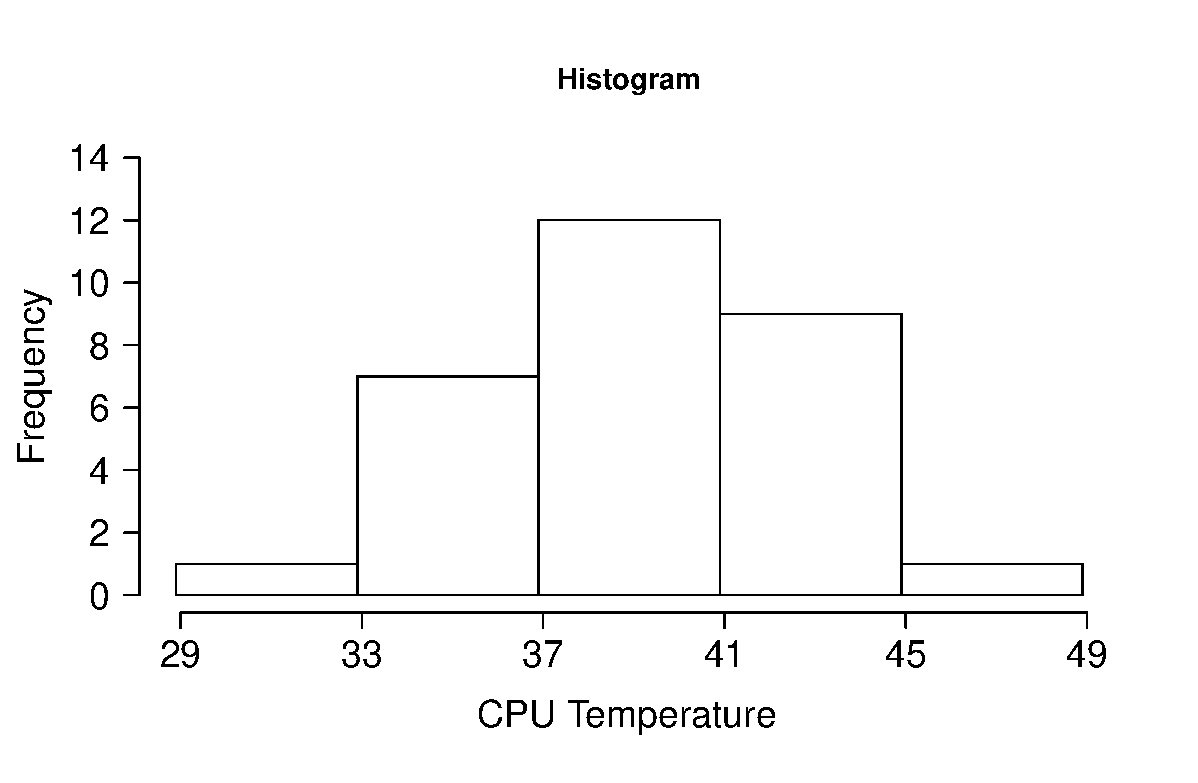
\includegraphics[width=0.9\textwidth, trim = 0.0cm 0.0cm 0.3cm 1.5cm, clip]{HistCPU}
\end{tabular}
\end{enumerate}
\end{minipage}\hspace{0.055\textwidth}
\begin{minipage}[t]{0.47\textwidth}
\quad

\begin{tabular}{c|c|c}
 & {\bf Position} & {\bf Value} \\[0.1cm]
$Q_1$ & $\tfrac{n+1}{4} = \tfrac{31}{4} = 7.75$ & $\tfrac{36.7+36.8}{2} = {\bf36.75}$\\[0.3cm]
$Q_2$ & $\tfrac{n+1}{4}\times2 = 7.75(2) = 15.5$ & $\tfrac{39.3+39.6}{2} = {\bf39.45}$\\[0.3cm]
$Q_3$ & $\tfrac{n+1}{4}\times3 = 7.75(3) = 23.25$ & $\tfrac{41.4+41.6}{2} = {\bf41.5}$\\
\multicolumn{3}{c}{}\\
\end{tabular}
\begin{enumerate}
\item[c)] The median is $Q_2 = 39.45.$
\item[d)] The quartiles are $Q_1 = 36.75$, $Q_2 = 39.45$ and $Q_3 = 41.5.$
\item[e)] $IQR = Q_3 - Q_1 = 41.5-36.75 = 4.75.$\\[-0.6cm]
\begin{align*}
LF &= Q_1 - 1.5 IQR \\
&= 36.75 - 1.5(4.75) = 29.625.\\[0.3cm]
UF &= Q_3 + 1.5 IQR \\
&= 41.5 + 1.5(4.75) = 48.625
\end{align*}
There are no numbers less than 29.625 or greater than 48.625
$\Rightarrow$ no outliers.
\item[f)]
\begin{tabular}{c}
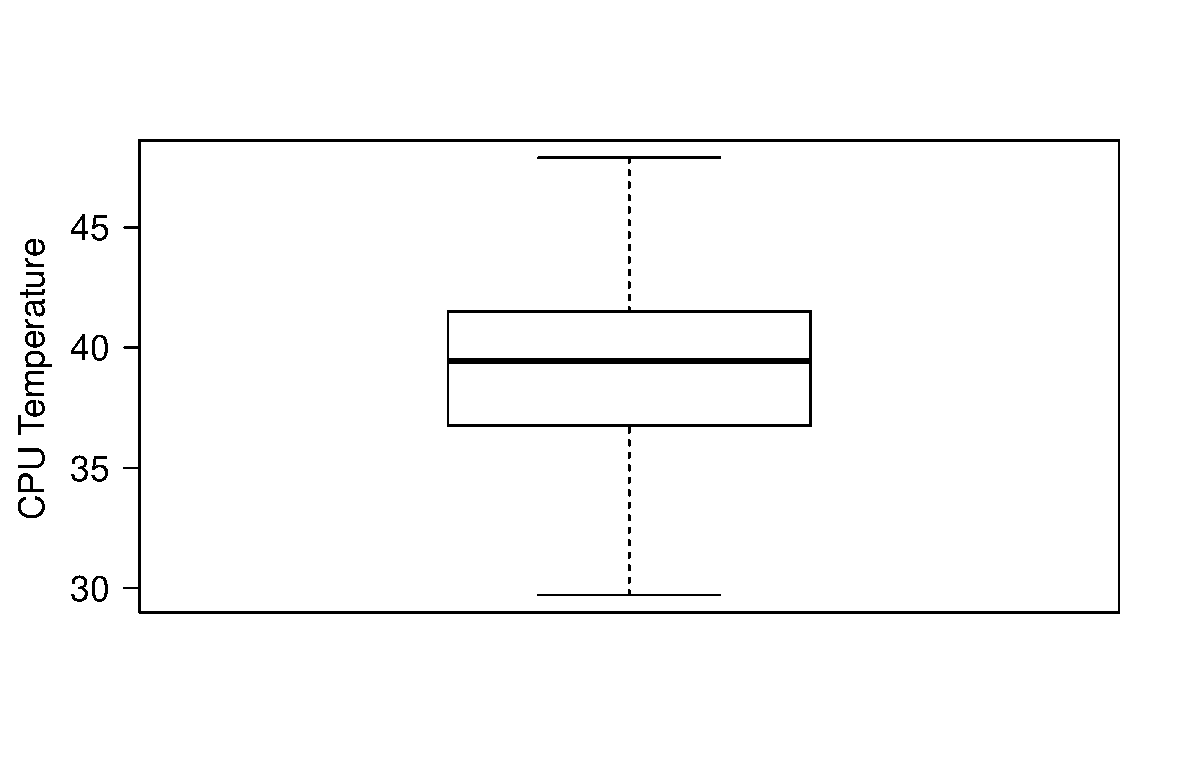
\includegraphics[width=0.9\textwidth, trim = 0.0cm 0.5cm 0.3cm 1.5cm, clip]{Bxp}\\
\end{tabular}
\item[g)] Based on the histogram and boxplot, we see that the data is symmetrical.
\end{enumerate}
\end{minipage}
\end{minipage}}\vspace{0.03\textwidth}



\end{document} 